\documentclass[border=7pt]{standalone}
\usepackage{amsmath,amssymb,bm,mathtools}
\usepackage[fontset=none]{ctex}
\setCJKmainfont{Songti SC}\setCJKsansfont{PingFang SC}
\usepackage{tikz}\usetikzlibrary{arrows.meta,calc,patterns,angles,quotes,decorations.markings,decorations.pathmorphing}
\newcommand{\dd}{\mathop{}\!\mathrm d}
\definecolor{blue}{HTML}{235789}\definecolor{red}{HTML}{BC4B41}
\tikzset{axis/.style={->,>=Stealth,line width=.55pt},world/.style={line width=.9pt},flow/.style={->,>=Stealth,line width=.85pt},ray/.style={->,>=Stealth,line width=.85pt},guide/.style={dashed,line width=.4pt},aux/.style={dashed,line width=.4pt},dim/.style={<->,>=Stealth,line width=.5pt},every node/.style={font=\normalsize},force/.style={->,>=Stealth,very thick},gas/.style={fill=blue!7}}
\begin{document}
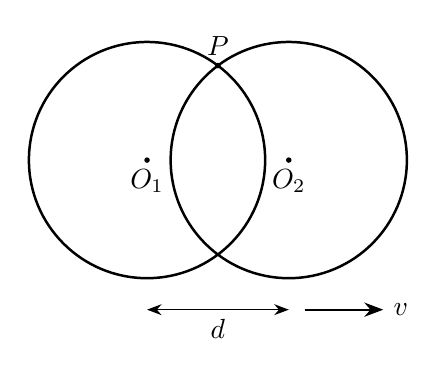
\begin{tikzpicture}\draw[world](0,0)circle(1.5) (1.8,0)circle(1.5);\fill(0,0)circle(1pt)node[below]{$O_1$};\fill(1.8,0)circle(1pt)node[below]{$O_2$};\fill(.9,1.2)circle(1pt)node[above]{$P$};\draw[dim](0,-1.9)--(1.8,-1.9)node[midway,below]{$d$};\draw[flow](2,-1.9)--(3,-1.9)node[right]{$v$};\end{tikzpicture}
\end{document}
